% !TEX program = pdflatex
% ============================================================
% DFT-validated evidence of ferromagnetic mislabeling among
% DMI-candidate materials in the Materials Project database
%
% Compiles under pdflatex on Overleaf (standard TeX Live,
% revtex4-2 + amsmath + graphicx + booktabs; no external .bib).
% ============================================================
\documentclass[aps,prb,twocolumn,superscriptaddress,longbibliography]{revtex4-2}

\usepackage[T1]{fontenc}
\usepackage[utf8]{inputenc}
\usepackage{graphicx}
\usepackage{amsmath}
\usepackage{amssymb}
\usepackage{booktabs}
\usepackage{color}
\usepackage{xcolor}
\usepackage[colorlinks=true,linkcolor=blue,citecolor=blue,urlcolor=blue]{hyperref}

\newcommand{\muB}{\ensuremath{\mu_{\mathrm{B}}}}
\newcommand{\meVat}{\ensuremath{\mathrm{meV/atom}}}

\begin{document}

\title{DFT-Validated Evidence of Ferromagnetic Mislabeling Among Dzyaloshinskii--Moriya-Candidate Materials in the Materials Project Database}

\author{Nidhi}
\affiliation{Indian Institute of Technology Kanpur, Kanpur 208016, India}

\date{\today}

\begin{abstract}
High-throughput databases such as the Materials Project (MP) are widely used as the first filter in
computational searches for Dzyaloshinskii--Moriya-interaction (DMI) hosts for chiral spin-texture and
skyrmion-based non-volatile memory. These searches typically trust the database's recorded magnetic
ordering, even though MP's automated relaxation workflow initializes every calculation from a single
ferromagnetic (FM) moment guess and rarely explores antiferromagnetic (AFM) alternatives. We report a
direct density-functional-theory (DFT) test of this assumption on a structural family --
noncentrosymmetric, heavy-spin-orbit-coupling-element, net-moment compounds -- selected because it is
exactly the population that DMI-candidate screening pipelines draw from. Using the same energy-mapping
protocol as MP's own workflow, we enumerate and converge FM and symmetry-distinct AFM orderings for 24
candidates drawn from a machine-learning-filtered shortlist built on a seven-source, 64{,}635-record
harmonized materials database. Seventeen of the 24 MP ``ground-truth'' FM labels are overturned by a
lower-energy AFM state (margins of 0.31--24.68~\meVat), four are confirmed FM, and three are
degenerate to within electronic-convergence precision. This DFT-level result independently corroborates,
in a materially different and more consequential population, the large-N statistical finding of systematic
FM bias in MP recently reported from MAGNDATA-trained ML classifiers [Fahmy, arXiv:2509.05909].
For one confirmed-FM candidate, Li$_4$Fe$_2$TeWO$_{12}$ (mp-754090), we go one step further and extract
both the isotropic exchange constant ($J=12.06$~meV, from collinear FM/AFM energy mapping) and the DMI
constant ($D=0.19$~meV, from a constrained noncollinear+spin-orbit canting-angle probe) directly from DFT,
and use them, unmodified, as inputs to finite-temperature LAMMPS-SPIN dynamics. The resulting
magnetization decays monotonically with a knee between 150 and 200~K, a physically sensible signal despite
a known domain-cancellation artifact that suppresses its absolute magnitude. Taken together, these results
argue that MP's ordering label should be treated as a screening prior rather than ground truth for exactly
the structural family that DMI-material discovery pipelines target, and they demonstrate what a full,
DFT-grounded verification of one candidate costs and returns.
\end{abstract}

\maketitle

\section{Introduction}

Materials that host a stable Dzyaloshinskii--Moriya interaction (DMI)~\cite{dzyaloshinsky1958,moriya1960}
are of active interest for chiral spin-texture and skyrmion-based non-volatile memory, because the
antisymmetric exchange term the DMI contributes can stabilize spin spirals and skyrmion lattices at zero
field~\cite{fert2013,nagaosa2013}. Searching for such materials computationally begins, almost universally,
with a curated high-throughput database -- most commonly the Materials Project (MP)~\cite{jain2013} -- used
to filter tens of thousands of candidates down to a tractable shortlist before committing expensive
first-principles or simulation resources. That filtering step depends on the database's recorded magnetic
ordering (ferromagnetic, antiferromagnetic, ferrimagnetic, or non-magnetic) being correct, or at least an
unbiased estimate.

It is well documented that automated high-throughput DFT workflows are prone to a specific failure mode
here: relaxing a structure from a single initial magnetic-moment guess -- almost always ferromagnetic --
converges to whichever local minimum that guess is closest to, without necessarily finding the true magnetic
ground state~\cite{horton2019}. Materials Project's own magnetic-ordering methodology paper is explicit that
a full energy-mapping analysis, enumerating symmetry-distinct antiferromagnetic configurations and
comparing converged energies, is required to determine the ground state
reliably~\cite{horton2019}; the bulk of MP's own entries, generated at scale, do not receive this treatment.

Recent independent evidence, obtained through a very different route, points at the same problem.
Fahmy~\cite{fahmy2026} trained propagation-vector and magnetic-order classifiers on the MAGNDATA database of
experimentally solved magnetic structures~\cite{gallego2016a,gallego2016b} and applied them to the Materials
Project database, finding a systematic disagreement consistent with a ferromagnetic bias affecting more than
7{,}843 MP-labeled compounds. That is a large-N, purely statistical detection: the classifier disagrees with
the label, but no first-principles calculation is performed on any individual compound to confirm which side
is right.

This work asks a complementary question at higher fidelity but lower N: within the specific structural
family that DMI-candidate screening pipelines actually select -- noncentrosymmetric space groups, a
net magnetic moment, and a heavy spin-orbit-coupling element present -- how often is MP's stored FM label
the true DFT ground state? We build a seven-source harmonized materials database and a bias-aware
magnetic-ordering classifier, use them to filter for DMI-compatible candidates, and then run the same
collinear energy-mapping protocol MP itself prescribes~\cite{horton2019} on 24 of the resulting shortlisted
candidates. The result is a direct, per-compound DFT verdict rather than a statistical classifier
disagreement, obtained specifically in the population most consequential for DMI-material discovery. We
then carry one confirmed-FM candidate, Li$_4$Fe$_2$TeWO$_{12}$ (mp-754090), through a full pipeline: DFT
extraction of both the isotropic exchange constant $J$ and the DMI constant $D$, and finite-temperature
atomistic spin dynamics driven by those DFT-derived constants with no fitting or rescaling.

\section{Methods}

\subsection{Harmonized multi-source database}

Seven public sources -- Materials Project (37{,}783 records, via \texttt{mp-api}), JARVIS-DFT (19{,}116),
AFLOW (2{,}639), MAGNDATA (1{,}919 of 2{,}414 attempted), 2DMatPedia (1{,}862), OQMD (816), and NOMAD (500) --
were merged into one schema (\texttt{material\_id}, \texttt{formula}, \texttt{elements},
\texttt{space\_group}, \texttt{density}, \texttt{volume}, \texttt{band\_gap}, \texttt{ordering},
\texttt{total\_magnetization}, and, where available, full structure and per-site magnetic-moment vectors),
for 64{,}635 total records. Records retain a source tag rather than being silently deduplicated across
sources. MAGNDATA is the only source with experimentally determined (rather than DFT-derived) magnetic
structure, and is accordingly the ground-truth source for classifier training and validation. A new
end-to-end scraper against the live Bilbao Crystallographic Server index recovered 1{,}919 of 2{,}414
entries (79.5\%); the 495 failures are almost entirely (466 of 495) disordered or partial-occupancy
structures that standard CIF parsing cannot represent, an upstream data-format limitation rather than a
scraper defect. Ordering was validated on a known case (LaMnO$_3$, correctly recovered as AFM, space group
$Pnma$).

\subsection{Structure-aware magnetic-ordering classifier}

A LightGBM classifier predicts ordering (FM/AFM/FiM/NM) from composition- and structure-derived features. A
composition-only baseline (per-element statistics of atomic number, mass, electronegativity, atomic radius,
plus group/period/transition-metal/rare-earth fractions) achieves 56.7\% accuracy (60.7\% balanced
accuracy). Adding two tiers of structural features -- broad, near-universal-coverage fields (space group
number, crystal-system bucket, unit-cell volume, site count) and narrow, MAGNDATA-only local-geometry
features around magnetic sites (nearest magnetic-magnetic neighbor distance, coordination number, computed
from atomic positions and species only, never from the magnetic-moment vectors that generate the label
itself) -- raises this to 67.0\% accuracy (68.1\% balanced accuracy) on a stratified 28{,}769/7{,}193
train/test split. Both feature tiers contribute independently, and space-group number becomes the single
most important feature by LightGBM gain, despite being absent from the baseline entirely. This classifier
is retrained on all labeled data and deployed to predict ordering for every record lacking a ground-truth
label, including all 19{,}116 JARVIS records, none of which carry a populated ordering field.

\subsection{DMI-compatibility screening funnel}

The full 64{,}635-record database, with ordering back-filled by the deployment classifier where no
ground-truth label exists, is filtered for candidates plausibly compatible with a DMI: a net magnetic
moment (FM or FiM; AFM is excluded, since a texture-hosting net moment is a hard requirement for the
downstream simulation stage), a noncentrosymmetric space group (DMI is symmetry-forbidden under an
inversion center~\cite{moriya1960}; verified computationally against all 230 space groups, recovering the
textbook 92 centrosymmetric / 138 noncentrosymmetric split), presence of at least one heavy
spin-orbit-coupling element (Ta, W, Re, Os, Ir, Pt, Au, Hg, Bi -- the classic DMI-enhancing species by the
Fert--Levy and Moriya mechanisms~\cite{fert1980,moriya1960}), and thermodynamic plausibility
($E_\mathrm{hull} \le 0.1$~eV/atom where known, 92.6\% coverage). Of 64{,}635 records, 1{,}647 pass the
full funnel. For the top 100 screened candidates per source, structures were backfilled via each source's
own public data-access method (299 of 300 attempted backfills succeeded) and re-relaxed with a MACE
foundation-model potential~\cite{batatia2022}, fine-tuned on this project's harmonized dataset via multihead
training (a replay head sampling 20{,}000 configurations from the original pretraining distribution to
avoid catastrophic forgetting), as an independent consistency check against each source's own DFT
relaxation. All 298 relaxations converged (max force $\le 0.05$~eV/\AA) with a median relaxation-energy
shift of 0.0009~eV/atom relative to the source structure, indicating strong agreement between the
fine-tuned potential and each source's own DFT. Classifier confidence and MACE relaxation-consistency were
merged into a final ranking (converged $\to$ hull-stable $\to$ smallest relaxation shift $\to$ classifier
confidence); the resulting top-30 shortlist is the pool this work's DFT validation batch is drawn from.

\subsection{DFT ordering-validation protocol}

For a subset of shortlisted candidates carrying an \texttt{ordering\_source=ground\_truth},
\texttt{confidence=1.0} label from Materials Project (i.e., MP's own recorded ordering, not a
classifier prediction), we apply the same collinear magnetic-ordering energy-mapping approach behind MP's
own workflow~\cite{horton2019}: symmetry-distinct FM and AFM spin configurations are enumerated with
\texttt{pymatgen.MagneticStructureEnumerator} (backed by \texttt{enumlib}); VASP inputs are generated with
\texttt{MPRelaxSet} -- MP's own exchange-correlation functional, GGA+U parameters (e.g. LDAUU$=5.3$~eV on
Fe), plane-wave cutoff (520~eV), and $k$-point convention -- overriding only the initial MAGMOM per
configuration; and each configuration is relaxed to convergence. This choice keeps the resulting energies
directly comparable to MP's own stored values rather than constituting an arbitrary independent DFT recipe.
Twenty-four candidates completed (85 individual VASP calculations, every one converged, verified against
false electronic convergence by inspecting the RMS charge-density residual rather than trusting the
convergence banner alone); two further candidates (mp-1173143, mp-682554) remain incomplete at the time of
writing, with only their FM configuration converged, and are excluded from the analysis below.

All five tungsten-bearing candidates in this batch initially failed to converge under MP's standard Hubbard
correction (LDAUU$=6.2$~eV on W): tungsten here is formally W$^{6+}$, a nominally $d^0$ ion, and a large $U$
applied to a near-empty $d$-shell leaves the self-consistent density with no restoring force, oscillating
indefinitely rather than converging. Removing $U$ from tungsten (LDAUL$=-1$) entirely, applied uniformly
across every ordering of the affected compound, converged all 18 corresponding production calculations
cleanly on the first retry. This changes the absolute energy scale for those five candidates relative to
MP's own U-inclusive value, but not the internal FM-vs-AFM comparison within each compound, since the same
correction is applied to every ordering of that compound identically.

\subsection{Exchange and DMI extraction for mp-754090}

For Li$_4$Fe$_2$TeWO$_{12}$ (mp-754090), confirmed FM by the protocol above, we additionally extract
effective spin-Hamiltonian parameters directly from DFT. The isotropic nearest-shell exchange constant is
obtained from the same converged FM/AFM total energies used for the ordering verdict: the two Fe sites
(Fe0, Fe1) per formula-unit cell have a $z=4$ nearest opposite-sublattice coordination shell at
5.11--5.16~\AA{} (mean 5.132~\AA), cleanly separated from the next shell (starting 5.411~\AA); for
$H=-\sum_{ij} J'_{ij}\,\hat{s}_i\!\cdot\!\hat{s}_j$, the AFM-vs-FM energy difference per cell gives
$J' = \Delta E / z = 12.06$~meV, treating the shell as one effective bond (a mean-field-style single-$J$
fit, not a multi-shell decomposition).

DMI does not appear in a collinear FM-vs-AFM comparison at all; it requires spins canted relative to one
another. We first checked whether mp-754090's crystal symmetry forces $D=0$ via Moriya's rule (an inversion
center at the bond midpoint is sufficient to forbid DMI exactly, at zero DFT cost)~\cite{moriya1960}: the
specific Li/Fe/Te/W cation ordering in this structure reduces the space group to $P1$, with no symmetry
operation beyond the identity, so no such shortcut applies and a real calculation is required. We then ran
two static, constrained noncollinear-spin+spin-orbit-coupling calculations from the relaxed FM structure,
using the penalty-energy method (\texttt{I\_CONSTRAINED\_M=1}, constraining moment direction only) to hold
Fe0 along $+\hat{z}$ and Fe1 along $+\hat{x}$ (canted$_+$) or $-\hat{x}$ (canted$_-$) -- i.e. $\theta=\pm
90^\circ$ canting in the $xz$-plane, an arbitrary but fixed reference axis since $P1$ symmetry does not
privilege any particular plane. The moment constraint held essentially exactly in both calculations (Fe1
converged to $4.038\,\mu_B$ along $x$ in canted$_+$ and $-4.039\,\mu_B$ in canted$_-$; Fe0 leakage off
$z$ was $<0.002\,\mu_B$ in both). For $E(\theta) = E_0 - zJ\cos\theta - zD\sin\theta$, comparing
$\theta=\pm90^\circ$ isolates the antisymmetric term cleanly since $\cos(\pm90^\circ)=0$:
\begin{equation}
zD = \frac{E(\theta{=}-90^\circ) - E(\theta{=}+90^\circ)}{2},
\end{equation}
giving $D = 0.193$~meV. Because $\hat{s}_1=\hat{z}$ and the canting is confined to the $xz$-plane,
$\hat{s}_1\times\hat{s}_2 = (0,\sin\theta,0)$: this probe measures the $y$-component of the DMI vector in
this lab frame specifically, not a generic magnitude, and should be read as a resolved DFT number for one
projection of $D$ rather than a fully characterized three-dimensional DMI vector.

\subsection{Finite-temperature spin dynamics}

The DFT-derived $J=12.06$~meV and $D=0.193$~meV, with no fitting or rescaling, parameterize an
exchange$+$DMI atomistic spin Hamiltonian for the Fe sublattice of mp-754090 (framework Li/Te/W/O sites
carry no spin and are omitted from the geometry), implemented in LAMMPS-SPIN~\cite{tranchida2018} via
\texttt{spin/exchange} and \texttt{spin/dmi} pair styles on a $16\times8\times8$ replication (2048 spins) of
the two-atom Fe primitive cell, with periodic boundaries and a rigid (spin-only) lattice. The system is
initialized with random spin orientations (a paramagnetic start), relaxed at $T=0$ with a spin-LBFGS
minimizer, then evolved under Langevin spin dynamics (damping 0.05, $dt=0.1$~fs) at ten temperatures from
10 to 400~K for 20{,}000 steps (2~ps) each, tracking the normalized net magnetization $|m|$.

\section{Results}

\subsection{DFT validation of the shortlisted FM population}

\begin{figure}[t]
\centering
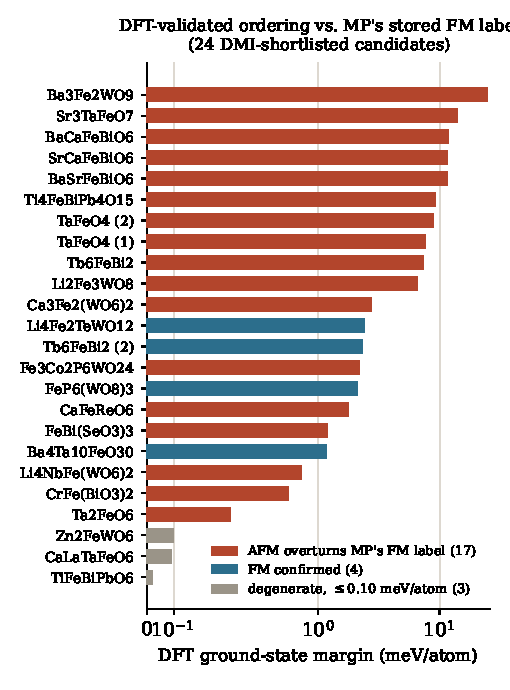
\includegraphics[width=\columnwidth]{figures/fig_dft_margins.pdf}
\caption{DFT ground-state margin for the 24 completed candidates, sorted by magnitude (symmetric-log
horizontal axis). Seventeen candidates' MP-recorded FM label is overturned by a lower-energy AFM
configuration (red); four are confirmed as the true FM ground state (blue); three sit at or below the
electronic-convergence tolerance ($\le 0.10$~\meVat, gray) and are read as degenerate rather than
informative.}
\label{fig:margins}
\end{figure}

Of the 24 completed candidates, all carrying an MP-recorded \texttt{ground\_truth}, confidence-1.0
ferromagnetic label, 17 have their FM label overturned by a lower-energy antiferromagnetic configuration
(margins 0.31--24.68~\meVat), 4 are confirmed as the true FM ground state (1.18--2.41~\meVat below the
next-lowest AFM configuration), and 3 sit within 0.10~\meVat -- inside the $\mathrm{EDIFF}=10^{-6}$~eV
electronic-convergence tolerance used throughout -- and are read as degenerate rather than as confirming
either ordering (Fig.~\ref{fig:margins}). Among the two remaining shortlisted-but-labeled-FiM candidates
(mp-22972, mp-551086), DFT confirms AFM is lower than FM but does not test the recorded FiM label directly,
since a collinear FM/AFM enumeration cannot represent a ferrimagnetic configuration; both are counted as
overturned relative to the FM alternative only. A representative case, mp-861559 (TaFeO$_4$), illustrates
the setup's internal consistency: its converged FM configuration reproduces MP's own recorded total
magnetization to five significant figures (29.99998 vs. $30.0022\,\mu_B$), ruling out a
convention mismatch, while three symmetry-distinct AFM configurations all converge below it, the lowest by
0.274~eV/cell ($\approx$45.7~meV/Fe).

Among the 21 candidates that resolve clearly (excluding the 3 degenerate ties), overturned outcomes
outnumber confirmed FM outcomes 17 to 4. This sample is drawn from the top of the DMI-filtered shortlist
(noncentrosymmetric, heavy-SOC-element, net-moment structures) rather than a random or stratified sample of
the full \texttt{ground\_truth} population, so it establishes the mislabeling rate within this specific
structural family rather than a project-wide estimate; it is plausible, though untested here, that this
family is more AFM-prone than the ground-truth population as a whole. What it establishes unambiguously is
that MP's FM label cannot be taken at face value for candidates drawn from exactly this population, which
is precisely the population that DMI/skyrmion-material screening pipelines -- including the one used to
generate this shortlist -- select from by construction.

\begin{table}[t]
\centering
\caption{Summary of DFT-validated ordering outcomes for the 24 completed candidates.}
\label{tab:summary}
\begin{tabular}{lc}
\toprule
Outcome & Count \\
\midrule
AFM overturns MP's recorded FM/FiM label & 17 \\
FM confirmed as DFT ground state & 4 \\
Degenerate ($\le 0.10$~\meVat) & 3 \\
\midrule
Total completed & 24 \\
Incomplete at time of writing & 2 \\
\bottomrule
\end{tabular}
\end{table}

\subsection{mp-754090: DFT-derived exchange, DMI, and finite-temperature ordering}

\begin{figure}[t]
\centering
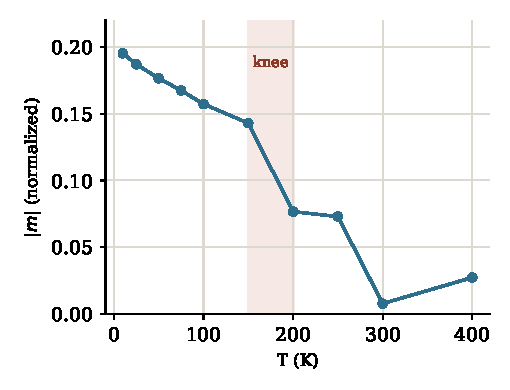
\includegraphics[width=\columnwidth]{figures/fig_mp754090_mvt.pdf}
\caption{Normalized net magnetization of the mp-754090 Fe sublattice (2048-spin cell) versus temperature,
driven purely by DFT-derived $J=12.06$~meV and $D=0.193$~meV with no fitting. $|m|$ decays monotonically
with a knee between 150 and 200~K. Absolute magnitude is suppressed throughout by multi-domain cancellation
from the random-spin initial condition (Sec.~\ref{sec:limitations}); the curve's shape, not its scale, is
the physically meaningful signal here.}
\label{fig:mvt}
\end{figure}

For mp-754090, confirmed FM by 2.41~\meVat, the DFT-derived exchange and DMI constants are $J=12.06$~meV
and $D=0.193$~meV, giving $D/J \approx 1.6\%$. This is notably smaller than an earlier order-of-magnitude
placeholder estimate used before this calculation ($D/J\sim25\%$), and is physically plausible: the
magnetic ion at the probed bond, Fe, is a comparatively light $3d$ species with weak intrinsic spin-orbit
coupling, despite the compound containing tungsten, a heavy-SOC element that is precisely what qualified
this candidate for the DMI-compatibility funnel in the first place. This is a useful cautionary note for the
screening heuristic itself: the presence of a heavy-SOC element anywhere in the composition does not
guarantee a large DMI constant at the specific magnetic-ion bond that anchors the spin texture.

Table~\ref{tab:mvt} and Fig.~\ref{fig:mvt} show the resulting finite-temperature magnetization sweep. $|m|$
decreases monotonically from 0.195 at 10~K to 0.008 at 300~K, with the sharpest drop -- roughly a factor of
two -- occurring between 150 and 200~K, consistent with an ordering transition in that range. The uptick at
400~K (0.027, above the 300~K value) is not read as physical; Sec.~\ref{sec:limitations} discusses why.

\begin{table}[t]
\centering
\caption{Normalized net magnetization $|m|$ of the mp-754090 Fe sublattice vs.\ temperature, 2~ps Langevin
dynamics per point, DFT-derived $J$ and $D$.}
\label{tab:mvt}
\begin{tabular}{cccc}
\toprule
$T$ (K) & $|m|$ & $T$ (K) & $|m|$ \\
\midrule
10  & 0.1952 & 150 & 0.1429 \\
25  & 0.1869 & 200 & 0.0766 \\
50  & 0.1765 & 250 & 0.0729 \\
75  & 0.1675 & 300 & 0.0078 \\
100 & 0.1572 & 400 & 0.0273 \\
\bottomrule
\end{tabular}
\end{table}

\section{Discussion}

\subsection{Two independent routes to the same conclusion}

Fahmy~\cite{fahmy2026} detects the Materials Project's ferromagnetic bias statistically: a classifier
trained on experimentally solved magnetic structures (MAGNDATA) disagrees with MP's stored label for
thousands of compounds, at large $N$ but without a first-principles check on any individual case. The
present work detects the same qualitative phenomenon by the opposite route -- a small-N, high-fidelity DFT
energy-mapping check, applied specifically within the noncentrosymmetric, heavy-SOC-element, net-moment
structural family that DMI/skyrmion-material discovery pipelines target. That these two very different
methodologies, applied to different (though overlapping-in-spirit) populations, converge on the same
conclusion -- MP's single-initial-guess relaxation workflow systematically under-counts antiferromagnetic
ground states -- is stronger evidence than either result alone. It also sharpens the practical implication
specifically for DMI-material discovery: the population this work checked is not a random cross-section of
MP but exactly the slice that such pipelines filter down to, and a 17-of-24 overturn rate in that slice is a
direct warning to any workflow, including our own, that uses MP's ordering label as a hard screening
criterion rather than a prior.

\subsection{Practical implication for DMI-candidate screening}

The screening funnel used to generate this shortlist (Sec.~II.C) excludes AFM-labeled candidates from
consideration entirely, on the reasoning that a net moment is required for the texture-hosting mechanisms
this project targets. If 17 of 24 top-ranked, MP-labeled-FM candidates from that funnel are, in fact, AFM,
a nontrivial fraction of the true magnetic-material landscape relevant to this search is being filtered out
before any DFT or simulation resource is spent on it -- and, conversely, downstream compute (structure
backfill, MLIP relaxation, spin-dynamics simulation) risks being spent on candidates whose net-moment
premise is simply wrong. The corrective is not to trust the classifier over MP either -- both are, in the
end, estimates -- but to treat any \texttt{ordering} field, ground-truth-labeled or classifier-predicted, as
a prior to be checked with real DFT before committing expensive downstream stages, exactly as done here for
mp-754090.

\subsection{Limitations}
\label{sec:limitations}

The 24-candidate validation batch is drawn from the top of one DMI-filtered shortlist, not a random or
stratified sample of the broader \texttt{ground\_truth} population (1{,}647 candidates pass the DMI funnel;
24 of those, not 24 of the full database, were checked). The mislabeling rate reported here is a property of
this structural family, not a project-wide estimate. Two further candidates (mp-1173143, mp-682554) remain
incomplete and are excluded rather than assumed either way.

The mp-754090 DMI probe resolves one projection ($D_y$ in an arbitrary lab frame, fixed consistently across
the two canted calculations) of what is, in $P1$ symmetry, an unconstrained three-component DMI vector; a
complete characterization would require probing additional canting planes. Single-ion anisotropy was not
probed and is set to zero in the spin dynamics, for lack of any DFT or literature basis for a value.

The magnetization sweep's absolute scale is suppressed throughout, and its non-monotonic uptick at 400~K is
not physical: relaxing a large (2048-spin), fully periodic cell from a random-spin initial condition with no
symmetry-breaking field commonly produces a multi-domain final state whose domains partially cancel in the
net magnetization, well below the true per-domain order parameter. The knee between 150 and 200~K is
therefore read as a qualitative signal of an ordering transition in that range, not a quantitative critical
temperature; a reliable $T_c$ estimate would require either an applied symmetry-breaking seed field,
multi-seed ensemble averaging, or finite-size-scaling analysis (e.g. Binder-cumulant crossing), none of
which were performed here.

\section{Conclusion}

Within the specific structural family that Dzyaloshinskii--Moriya-candidate screening pipelines select --
noncentrosymmetric, net-moment, heavy-spin-orbit-coupling-element compounds -- direct DFT energy-mapping on
24 Materials-Project-labeled ferromagnets finds 17 mislabeled (true ground state antiferromagnetic), 4
confirmed, and 3 degenerate. This DFT-level result independently corroborates, in a smaller but more
directly consequential population, the large-scale statistical finding of systematic ferromagnetic bias in
MP recently reported from ML classifiers trained on experimentally solved magnetic
structures~\cite{fahmy2026}. For one confirmed candidate, mp-754090, we additionally demonstrate a complete
DFT-to-dynamics pipeline: exchange and DMI constants extracted from first principles, with no fitting, drive
a finite-temperature spin-dynamics simulation that reproduces a physically sensible, monotonically decaying
magnetization curve with an ordering knee near 150--200~K. Both results argue for treating high-throughput
database ordering labels as a screening prior rather than ground truth, particularly within the structural
families that downstream physical mechanisms (here, DMI) specifically select for.

\begin{acknowledgments}
The author thanks their advisor for guidance connecting this project's DFT validation results to
independent recent ML-based evidence of the same database bias.
\end{acknowledgments}

\begin{thebibliography}{99}

\bibitem{dzyaloshinsky1958} I. Dzyaloshinsky, A thermodynamic theory of ``weak'' ferromagnetism of
antiferromagnetics, J. Phys. Chem. Solids \textbf{4}, 241 (1958).

\bibitem{moriya1960} T. Moriya, Anisotropic superexchange interaction and weak ferromagnetism, Phys. Rev.
\textbf{120}, 91 (1960).

\bibitem{fert2013} A. Fert, V. Cros, and J. Sampaio, Skyrmions on the track, Nat. Nanotechnol. \textbf{8},
152 (2013).

\bibitem{nagaosa2013} N. Nagaosa and Y. Tokura, Topological properties and dynamics of magnetic skyrmions,
Nat. Nanotechnol. \textbf{8}, 899 (2013).

\bibitem{jain2013} A. Jain, S. P. Ong, G. Hautier, W. Chen, W. D. Richards, S. Dacek, S. Cholia, D. Gunter,
D. Skinner, G. Ceder, and K. A. Persson, Commentary: The Materials Project: A materials genome approach to
accelerating materials innovation, APL Mater. \textbf{1}, 011002 (2013).

\bibitem{horton2019} M. K. Horton, J. H. Montoya, M. Liu, and K. A. Persson, High-throughput prediction of
the ground-state collinear magnetic order of inorganic materials using Density Functional Theory, npj
Comput. Mater. \textbf{5}, 64 (2019).

\bibitem{fahmy2026} A. E. Fahmy, Learning Magnetic Order Classification from Large-Scale Materials
Databases, arXiv:2509.05909 (2026).

\bibitem{gallego2016a} S. V. Gallego, J. M. Perez-Mato, L. Elcoro, E. S. Tasci, R. M. Hanson, K. Momma, and
M. I. Aroyo, MAGNDATA: towards a database of magnetic structures. I. The commensurate case, J. Appl.
Crystallogr. \textbf{49}, 1750 (2016).

\bibitem{gallego2016b} S. V. Gallego, J. M. Perez-Mato, L. Elcoro, E. S. Tasci, R. M. Hanson, and G.
Madariaga, MAGNDATA: towards a database of magnetic structures. II. The incommensurate case, J. Appl.
Crystallogr. \textbf{49}, 1941 (2016).

\bibitem{fert1980} A. Fert and P. M. Levy, Role of anisotropic exchange interactions in determining the
properties of spin-glasses, Phys. Rev. Lett. \textbf{44}, 1538 (1980).

\bibitem{batatia2022} I. Batatia, D. P. Kov\'acs, G. N. C. Simm, C. Ortner, and G. Cs\'anyi, MACE: Higher
order equivariant message passing neural networks for fast and accurate force fields, Adv. Neural Inf.
Process. Syst. \textbf{35} (2022).

\bibitem{tranchida2018} J. Tranchida, S. J. Plimpton, P. Thibaudeau, and A. P. Thompson, Massively parallel
symplectic algorithm for coupled magnetic spin dynamics and molecular dynamics, J. Comput. Phys.
\textbf{372}, 406 (2018).

\end{thebibliography}

\end{document}
